% ====================================================================
% CS5296 Cloud Computing -- Spring 2026 -- Group 5 final report
%
% Compliant with the course style: A4, single column, single spaced,
% 12 pt Times New Roman. Page budget: 9 pages including references,
% excluding the Artifact Appendix.
% ====================================================================

\documentclass[a4paper,12pt]{article}

% --- Packages ---
\usepackage[margin=1in]{geometry}
\usepackage{mathptmx}                 % Times New Roman for text & math
\usepackage[utf8]{inputenc}
\usepackage[T1]{fontenc}
\usepackage[english]{babel}
\usepackage{graphicx}
\usepackage{booktabs}
\usepackage{hyperref}
\usepackage{url}
\usepackage{cite}
\usepackage{xcolor}
\usepackage{caption}
\usepackage{subcaption}
\usepackage{listings}
\usepackage{enumitem}
\usepackage{tikz}
\usetikzlibrary{positioning,fit,calc}
\usepackage{amsmath}
\usepackage{microtype}

% --- Layout tweaks ---
\setlength{\parskip}{2pt}
\setlength{\parindent}{0pt}
\setlength{\textfloatsep}{8pt plus 2pt minus 2pt}
\setlength{\floatsep}{8pt plus 2pt minus 2pt}
\setlength{\intextsep}{8pt plus 2pt minus 2pt}
\setlength{\abovecaptionskip}{4pt}
\setlength{\belowcaptionskip}{2pt}
\hypersetup{
  colorlinks = true,
  linkcolor  = blue!50!black,
  citecolor  = blue!50!black,
  urlcolor   = blue!50!black,
}

% --- IEEE-style numbering for sections, subsections and tables ------
\renewcommand{\thesection}{\Roman{section}}
\renewcommand{\thesubsection}{\thesection-\Alph{subsection}}
\renewcommand{\thetable}{\Roman{table}}

% --- Figure/table caption style (IEEE convention: bold label, then ".") ---
\captionsetup{labelfont=bf, labelsep=period, font=small}

% --- Title block --------------------------------------------------------
\title{\textbf{Baseline vs.\ Event-Driven Autoscaling in Kubernetes: \\
A Controlled Comparison of HPA and KEDA for a Queue-Backed Microservice}}
\author{%
  Group~5 \\
  \small CS5296 Cloud Computing, Spring 2026, City University of Hong Kong%
}
\date{April 2026}

\begin{document}
\maketitle

\begin{abstract}
Cloud-native microservices rely on elastic scaling to absorb volatile
workloads. Kubernetes ships two commonly used autoscalers: the
resource-based Horizontal Pod Autoscaler (HPA) and the event-driven
Kubernetes Event-Driven Autoscaling (KEDA) framework. We conduct a
controlled comparative study of the two on a RabbitMQ-backed Spring
Boot consumer deployed on a single-node K3s cluster hosted on an AWS
EC2 \texttt{m5.large} instance. Under an identical flash-crowd workload
(a 10~s burst targeting 1\,000~messages/s), three replications per group
are collected and compared along three axes: responsiveness,
user-visible effect, and resource utilisation. All non-signal scaling
parameters are held constant---in particular the \texttt{scaleDown}
\texttt{stabilizationWindowSeconds} is fixed at 60~s and the
\texttt{scaleDown} rate policy at 50\,\%/60~s for both groups. Under
this configuration, KEDA (queueLength signal) reacts $10.4$~s faster
than Baseline HPA (CPU signal) on average
($63.4 \pm 3.4$~s versus $73.8 \pm 8.3$~s), drains the backlog
$12.2$~s sooner, and begins to scale down $\approx$\,$327$~s after the
burst ends, whereas the Baseline HPA does not release any capacity
during the entire 355~s post-burst trial window. The root cause is
the signal's information asymmetry: CPU utilisation remains pinned at
the \texttt{limits.cpu} ceiling throughout the drain, structurally
preventing HPA from inferring a reduced workload, while queue length
decreases monotonically and thus serves as a leading indicator.
Within the observed window both groups still hit the same peak of six
pods and have near-identical pod-seconds overshoot, so KEDA's concrete
resource advantage is earlier capacity release rather than a lower peak
replica count. For queue-backed event-driven workloads,
queue-length-based autoscaling delivers measurable quality-of-service
gains that parameter tuning alone cannot recover.
\end{abstract}

\section{Introduction}
\label{sec:intro}

Elasticity is a core promise of cloud computing~\cite{mell2011nist}: applications should add capacity when demand rises and release it when demand falls. In many modern systems, demand does not arrive only as direct HTTP requests. It is often buffered through message queues, such as order-processing jobs during an e-commerce flash sale, telemetry events from Internet-of-Things devices, or asynchronous tasks in a machine-learning inference pipeline. In these workloads, the queue depth is an immediate measure of unfinished work. If the consumer deployment reacts late, users may experience long processing delays even though the cluster eventually scales out.

Kubernetes~\cite{kubernetes2024} provides the Horizontal Pod Autoscaler (HPA), which adjusts a Deployment's replica count so that a selected resource metric, usually CPU or memory utilisation, approaches a target value~\cite{kubernetes2024hpa}. HPA is simple and widely available, but CPU is an indirect and sometimes delayed signal for a queue-backed service. A consumer can be CPU-saturated while the backlog is either growing rapidly or almost drained; CPU alone does not tell the autoscaler how much work remains in the queue.

Kubernetes Event-Driven Autoscaling (KEDA)~\cite{keda2024} offers a different approach. Instead of asking only how busy the pods are, KEDA can ask how much work is waiting outside the pods. For RabbitMQ, KEDA can scale a consumer directly from queue length. Internally, KEDA still creates an HPA object, but the metric fed into the HPA is an external business metric rather than a CPU metric. This makes KEDA a useful comparison point for event-driven cloud workloads.

\textbf{Project nature and research question.} This is a technical cloud-computing project: we implement and evaluate existing autoscaling mechanisms rather than proposing a new autoscaling algorithm. The central question is: \emph{for the same RabbitMQ-backed consumer and the same burst workload, how do CPU-based HPA and queue-length-based KEDA differ in scale-up responsiveness, queue-drain performance, and scale-down behaviour?}

\textbf{Methodology.} We built a complete reproducibility artifact on GitHub~\cite{group5artifact2026}. The artifact deploys RabbitMQ, a Spring Boot consumer, HPA/KEDA policies, a Python load generator, and metric-collection scripts on a single-node K3s cluster. To make the comparison fair, both strategies use the same Docker image, CPU and memory requests/limits, minimum and maximum replica counts, and HPA \texttt{behavior} rules. The only independent variable is the signal used for scaling: CPU utilisation for HPA and RabbitMQ queue length for KEDA.

\textbf{Main findings.} KEDA reacts earlier, reaches useful capacity sooner, drains the queue faster, and is the only strategy that scales down during the observed post-burst window. The main reason is not that KEDA uses a more aggressive control loop. It uses a better signal for this workload. Queue length decreases continuously as work is completed, while CPU remains pinned near the pod limit as long as any backlog remains.

The rest of this report is organized as follows. Section~\ref{sec:background} reviews HPA and KEDA. Section~\ref{sec:design} presents the implemented system. Section~\ref{sec:setup} describes the experiment. Section~\ref{sec:results} analyzes the results. Section~\ref{sec:discussion} discusses implications and limitations, and Section~\ref{sec:conclusion} concludes.

\section{Background and Related Work}
\label{sec:background}

\subsection{Horizontal Pod Autoscaler}
\label{subsec:bg-hpa}
The Kubernetes HPA~\cite{kubernetes2024hpa} runs a reconciliation loop
with period controlled by the
\texttt{--horizontal-pod-autoscaler-sync-period} flag (15~s by
default). At each tick it queries \texttt{metrics-server}---itself
refreshed every 15~s from \texttt{kubelet}/cAdvisor---for the
target metric and computes the desired replica count via

\vspace{-6pt}
\begin{equation}
  \label{eq:hpa}
  n_\mathrm{desired} = \left\lceil n_\mathrm{current} \cdot
  \frac{m_\mathrm{current}}{m_\mathrm{target}} \right\rceil,
\end{equation}
\vspace{-8pt}

\noindent where $n_\mathrm{desired}$ is further clamped to the
$[\mathrm{minReplicas},\,\mathrm{maxReplicas}]$ range. A
\texttt{behavior} block governs how quickly the desired change takes
effect: \texttt{stabilizationWindowSeconds} computes the running
maximum over a rolling window (so transient dips do not immediately
trigger scale-down), while a \texttt{policies} list such as
\texttt{Percent 50\%/60s} caps the per-period scaling rate. When the
signal is \texttt{cpu.Utilization}, $m_\mathrm{current}$ is the mean CPU
usage divided by \texttt{requests.cpu}. Consequently, a pod whose CPU
is pinned at \texttt{limits.cpu} reports a utilisation equal to the
\emph{static} limit-to-request ratio rather than the \emph{dynamic}
load on the queue it serves---a structural limitation we revisit
in Section~\ref{sec:results}.

\subsection{Kubernetes Event-Driven Autoscaling}
\label{subsec:bg-keda}
KEDA~\cite{keda2024} is a CNCF graduated project that extends
Kubernetes with the \texttt{ScaledObject} custom resource. It ships
with more than 60 scalers for message brokers, databases, HTTP
endpoints, and custom sources~\cite{keda2024scalers}, and internally
materialises a hidden HPA whose target metric is of type
\texttt{External} and is served by the KEDA metrics adapter. Thus the
control \emph{mechanism} is identical to the standard HPA; the only
additional machinery is a short-lived metric pipeline that translates
a business signal (for example, RabbitMQ queueLength) into a scaling
ratio that Eq.~\ref{eq:hpa} can consume. For a
\texttt{rabbitmq/QueueLength} trigger the operator specifies a
messages-per-replica target~$T$, and KEDA reports
$m_\mathrm{current}/m_\mathrm{target} = Q/T$, where $Q$ is the
instantaneous queue depth. The desired replica count therefore
simplifies to $\lceil Q / T \rceil$, independent of CPU usage.

\subsection{Related Work}
\label{subsec:bg-related}
Prior work spans surveys of reactive and predictive autoscaling
algorithms~\cite{qu2018taxonomy}, Kubernetes-focused elasticity
benchmarks~\cite{nguyen2020hpa, medel2016modelling}, and event-driven
or serverless scaling studies~\cite{shahrad2020serverless}. What is
less common is a tightly controlled, same-hardware comparison between a
CPU-driven HPA baseline and a business-metric-driven controller. The
present study narrows the scope deliberately: application, broker,
hardware, \texttt{behavior} block, and load pattern are held constant,
so the only independent variable is the scaling signal itself.

\section{System Design}
\label{sec:design}

\subsection{Architecture Overview}
\label{subsec:arch}
Fig.~\ref{fig:arch} depicts the end-to-end deployment. A single AWS
EC2 \texttt{m5.large} instance ($2$\,vCPU, $8$\,GiB RAM) hosts a
lightweight K3s~\cite{rancher2024k3s} v1.30 cluster with three
application namespaces: \texttt{rabbitmq} for the shared broker and
\texttt{baseline}/\texttt{keda} for the two experiment groups. The
\texttt{keda} namespace also hosts the KEDA operator and metrics
adapter installed by Helm. A
Python producer running on the evaluator's workstation injects load
into either \texttt{baseline-queue} or \texttt{keda-queue} over AMQP.
A shell-based collector (\texttt{scripts/collect-metrics.sh}) polls
the RabbitMQ Management API~\cite{broadcom2024rabbitmq} and
\texttt{kubectl} at $\approx$\,$1$~Hz and writes per-second
comma-separated-value (CSV) rows; the same script runs for both
groups so the observation pipeline is identical.

\begin{figure}[t]
  \centering
  % End-to-end architecture. Drawn in TikZ so it scales cleanly in PDF.
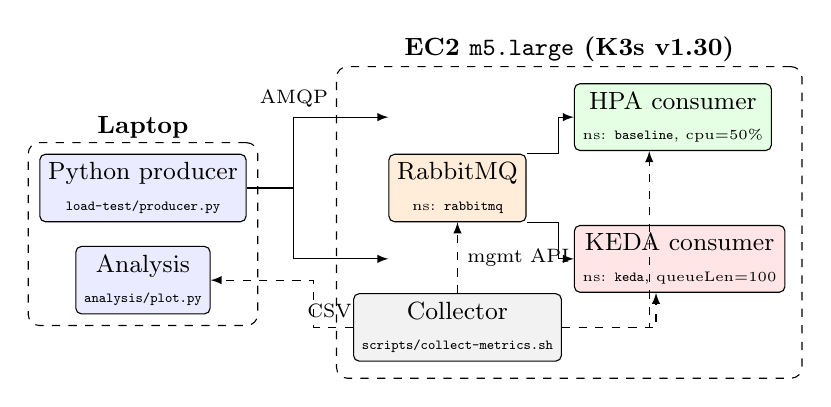
\begin{tikzpicture}[
  font=\small,
  box/.style={draw, rounded corners=2pt, align=center, inner sep=3pt,
              minimum height=7mm},
  node distance=3mm and 5mm,
]

% ---------- Laptop (load generator + analysis) ----------
\node[box, fill=blue!8]                         (producer) {Python producer\\{\tiny \texttt{load-test/producer.py}}};
\node[box, fill=blue!8, below=of producer]      (analysis) {Analysis\\{\tiny \texttt{analysis/plot.py}}};
\node[draw, dashed, rounded corners, fit=(producer) (analysis),
      inner sep=4pt, label={[yshift=-2pt]above:\textbf{Laptop}}] (laptop) {};

% ---------- EC2 node ----------
\node[box, fill=orange!15, right=18mm of producer] (rmq)      {RabbitMQ\\{\tiny ns: \texttt{rabbitmq}}};

\node[box, fill=green!10, right=6mm of rmq, yshift=9mm]  (base) {HPA consumer\\{\tiny ns: \texttt{baseline}, cpu=50\%}};
\node[box, fill=red!10,   right=6mm of rmq, yshift=-9mm] (keda) {KEDA consumer\\{\tiny ns: \texttt{keda}, queueLen=100}};

\node[box, fill=gray!10, below=9mm of rmq]     (collect)  {Collector\\{\tiny \texttt{scripts/collect-metrics.sh}}};

\node[draw, dashed, rounded corners,
      fit=(rmq) (base) (keda) (collect),
      inner sep=6pt,
      label={[yshift=-2pt]above:\textbf{EC2 \texttt{m5.large} (K3s v1.30)}}] (ec2) {};

% ---------- Arrows ----------
\draw[-latex] (producer.east) -- ++(0.6,0) |- (rmq.west |- base) node[midway, above,
      font=\scriptsize] {AMQP};
\draw[-latex] (producer.east) -- ++(0.6,0) |- (rmq.west |- keda);

\draw[-latex] (rmq.north east) -- ++(0.4,0) |- (base.west);
\draw[-latex] (rmq.south east) -- ++(0.4,0) |- (keda.west);

\draw[-latex, dashed] (collect.north) -- (rmq.south) node[midway, right,
      font=\scriptsize] {mgmt API};
\draw[-latex, dashed] (collect.east) -| ($(base.south)+(-3mm,0)$);
\draw[-latex, dashed] (collect.east) -| ($(keda.south)+(-3mm,0)$);

\draw[-latex, dashed] (collect.west) -- ++(-5mm,0)
      node[pos=0.6, above, font=\scriptsize] {CSV} |- (analysis.east);

\end{tikzpicture}

  \caption{End-to-end architecture on a single AWS EC2 node. The
  consumer image is shared by both groups; the only variable between
  them is the scaling policy attached to each Deployment.}
  \label{fig:arch}
\end{figure}

\subsection{Consumer Application}
\label{subsec:consumer}
Both groups run the same Spring Boot~\cite{vmware2024springboot}
consumer image (\texttt{htasteqin/cs5296-consumer:v1.0}). Each message
triggers a $\approx$\,$200$\,ms busy-wait so that the workload is
CPU-bound. This is a deliberate design choice: a
\texttt{Thread.sleep} would render HPA blind to the workload---since
the only available signal is CPU utilisation---and would therefore
bias the comparison before it begins. The pod resource settings are
\texttt{requests: 100m~CPU / 256~MiB} and
\texttt{limits: 300m~CPU / 512~MiB}.

\subsection{Scaling Strategies}
\label{subsec:strategies}
The two scalers share identical \texttt{minReplicas}$\,=\,$1 and
\texttt{maxReplicas}$\,=\,$6 (dictated by the 2\,vCPU node), together
with an identical \texttt{behavior} block:

\begin{itemize}[leftmargin=*,itemsep=0pt,topsep=1pt]
  \item \texttt{scaleUp}: \texttt{stabilizationWindowSeconds}\,=\,0;
        policies \texttt{Percent 100\%/15s} $\cup$
        \texttt{Pods 4/15s}, \texttt{selectPolicy}\,=\,\texttt{Max}.
  \item \texttt{scaleDown}: \texttt{stabilizationWindowSeconds}\,=\,60\,s;
        policy \texttt{Percent 50\%/60s}.
\end{itemize}

\noindent Only the scaling \emph{signal} differs:
\textbf{Baseline HPA} uses \texttt{cpu.Utilization} with a
$50\%$ target; \textbf{KEDA} uses a \texttt{rabbitmq}
\texttt{QueueLength} trigger with target~$T\,=\,100$
messages/replica and \texttt{pollingInterval}\,=\,5\,s.

\subsection{Control Variables}
\label{subsec:controls}
To isolate the effect of the scaling signal we hold all non-signal
parameters constant across the two groups: identical Docker image,
identical \texttt{requests}/\texttt{limits}, identical
$\approx$\,$200$\,ms per-message processing cost, a shared RabbitMQ
broker (separate queues per group to prevent interference), the same
EC2 node, and the same burst pattern. The only independent variable
is therefore the scaling signal---CPU utilisation versus queue
length.

\section{Experimental Setup}
\label{sec:setup}

\subsection{Environment}
\label{subsec:env}
\begin{itemize}[leftmargin=*,itemsep=0pt,topsep=1pt]
  \item \textbf{Cloud}: AWS EC2 \texttt{m5.large} ($2$\,vCPU,
        $8$\,GiB RAM, \texttt{us-west-2}), Ubuntu~22.04~LTS.
  \item \textbf{Cluster}: K3s v1.30 (single-node, embedded SQLite
        data store), Helm~3, \texttt{metrics-server} v0.7, and
        KEDA~v2.13 installed via its official Helm chart.
  \item \textbf{Broker}: a repository-owned RabbitMQ
        \texttt{StatefulSet} using image \texttt{rabbitmq:3.12-management},
        with \texttt{limits.cpu}\,=\,$1\,000$\,m,
        \texttt{limits.memory}\,=\,$1$\,GiB, and
        \texttt{tcpSocket:5672} readiness/liveness probes to avoid
        false failures on the constrained node.
\end{itemize}

\subsection{Workload}
\label{subsec:workload}
The pattern defined in
\texttt{load-test/patterns/burst.yaml} consists of three phases:
a $10$\,s warm-up at $5$\,messages/s (so that the collector captures
a steady-state baseline at \texttt{replicas}\,=\,1), a $10$\,s burst
\emph{targeting} $1\,000$\,messages/s, and $180$\,s of silence. The
harness script \texttt{run-experiment.sh} also waits $10$\,s before
launching the producer so the collector can record a baseline, and
then appends a further $180$\,s post-burst observation window. Each
trial therefore lasts $\approx$\,$390$\,s wall-clock, with roughly
$355$--$360$\,s of observation after the burst ends.

\paragraph{Producer ceiling.}~The
\texttt{pika}~\cite{pika2024} \texttt{BlockingConnection.basic\_publish}
call is a synchronous RPC that saturates at $\approx$\,$740$\,msg/s on
the \texttt{m5.large} node; consequently, the realised burst injects
$7\,100$--$7\,500$ messages rather than the nominal $10\,000$. The
ceiling affects both groups identically---the same producer publishes
to both queues with the same pattern---so it does not bias the
comparison.

\subsection{Metrics and Collection}
\label{subsec:metrics}
The collector \texttt{scripts/collect-metrics.sh} polls
\texttt{kubectl} for pod readiness and the RabbitMQ Management API
for queue statistics, emitting an 8-column CSV (see
artifact appendix). We derive three metric axes:

\begin{itemize}[leftmargin=*,itemsep=0pt,topsep=1pt]
  \item \textbf{Responsiveness.} Reaction latency (burst start
        $\rightarrow$ first new pod Ready), scale-up time (burst start
        $\rightarrow$ peak pod count), and drain time (burst end
        $\rightarrow$ \texttt{queue\_depth}\,=\,0).
  \item \textbf{User-visible effect.} Average delivery rate during the
        drain window and total messages delivered per trial.
  \item \textbf{Resource utilisation.} Scale-down-start time (burst end
        $\rightarrow$ first pod removal), pods still Ready at the end
        of the trial ($\approx$\,$355$\,s post-burst), and
        pod-seconds overshoot, defined as
        $\int \max\{0,\,\mathrm{pods}(t) - \mathrm{minReplicas}\}\,dt$
        over the entire trial.
\end{itemize}

\subsection{Trial Protocol}
\label{subsec:protocol}
For each of the two groups we run $n\,=\,3$ independent trials and
report the sample mean with one sample standard deviation. Between
trials the Deployment is scaled back to $1$ replica and the target
queue is purged. Each archived raw CSV therefore corresponds to the
same procedure: reset deployment, purge queue, capture a baseline,
run the burst pattern, then observe the drain and any scale-down.
All six formal trials were executed sequentially on 2026-04-20 and the
committed artefacts under \texttt{results/raw/} are the ground truth
for the statistics reported in this paper.

\section{Results and Analysis}
\label{sec:results}

All results are computed from the six trial CSV files in \path{results/raw/} using the analysis script \path{analysis/plot.py}. Unless stated otherwise, each value is the mean over three runs, with one sample standard deviation. Lower values are better for latency, scale-up time, and drain time; lower final pod counts are better after the workload has stopped.

\subsection{Headline Metrics}
\label{subsec:res-summary}
Table~\ref{tab:summary} shows the aggregate results. KEDA wins on all responsiveness metrics and is the only strategy that releases capacity before the observation window ends. The two strategies reach the same peak of six pods, so the difference is not maximum capacity. The difference is how early each strategy receives useful information about the burst and about the remaining backlog.

\begin{table}[t]
  \centering
  \small
  \caption{Headline metrics per strategy (mean $\pm$ standard deviation, $n=3$). ``---'' means the event was not observed within the trial window.}
  \label{tab:summary}
  \begin{tabular}{lcc}
    \toprule
    \textbf{Metric} & \textbf{HPA: CPU signal} & \textbf{KEDA: queue signal} \\
    \midrule
    \multicolumn{3}{l}{\emph{Responsiveness}} \\
    Reaction latency (s)                  & $73.8 \pm 8.3$   & $\mathbf{63.4 \pm 3.4}$ \\
    Time to peak pods (s)                 & $90.2 \pm 4.6$   & $\mathbf{80.2 \pm 5.1}$ \\
    Queue drain time (s)                  & $309.7 \pm 5.2$  & $\mathbf{297.6 \pm 5.6}$ \\
    \midrule
    \multicolumn{3}{l}{\emph{User-visible effect}} \\
    Avg. throughput during drain (msg/s)  & $22.75 \pm 0.27$ & $\mathbf{23.35 \pm 0.27}$ \\
    Messages delivered per trial          & $7\,451 \pm 57$  & $7\,212 \pm 90$ \\
    \midrule
    \multicolumn{3}{l}{\emph{Resource use}} \\
    First scale-down (s after burst end)  & ---              & $\mathbf{326.9 \pm 3.1}$ \\
    Ready pods at trial end               & $6.0$            & $\mathbf{3.0}$ \\
    Pod-seconds overshoot                 & $1\,426 \pm 27$  & $\mathbf{1\,415 \pm 7}$ \\
    Peak pod count                        & $6$              & $6$ \\
    \bottomrule
  \end{tabular}
\end{table}

The total delivered-message count should be interpreted as descriptive rather than as a direct performance score, because the actual number of messages published varies slightly with producer-side timing. Queue-drain time and delivery throughput are more comparable across runs because they normalize behaviour over the observed drain period.

\subsection{Responsiveness}
\label{subsec:res-response}
Fig.~\ref{fig:response} visualizes the three latency-style metrics. Compared with the CPU-based HPA, KEDA reacts 10.4~s earlier on average, which is a 14\% reduction in reaction latency. It also reaches the maximum useful replica count about 10~s earlier and clears the queue 12.2~s earlier. These differences are operationally meaningful: in a queue-backed service, every second of delayed scale-out allows the backlog to grow further.

\begin{figure}[t]
  \centering
  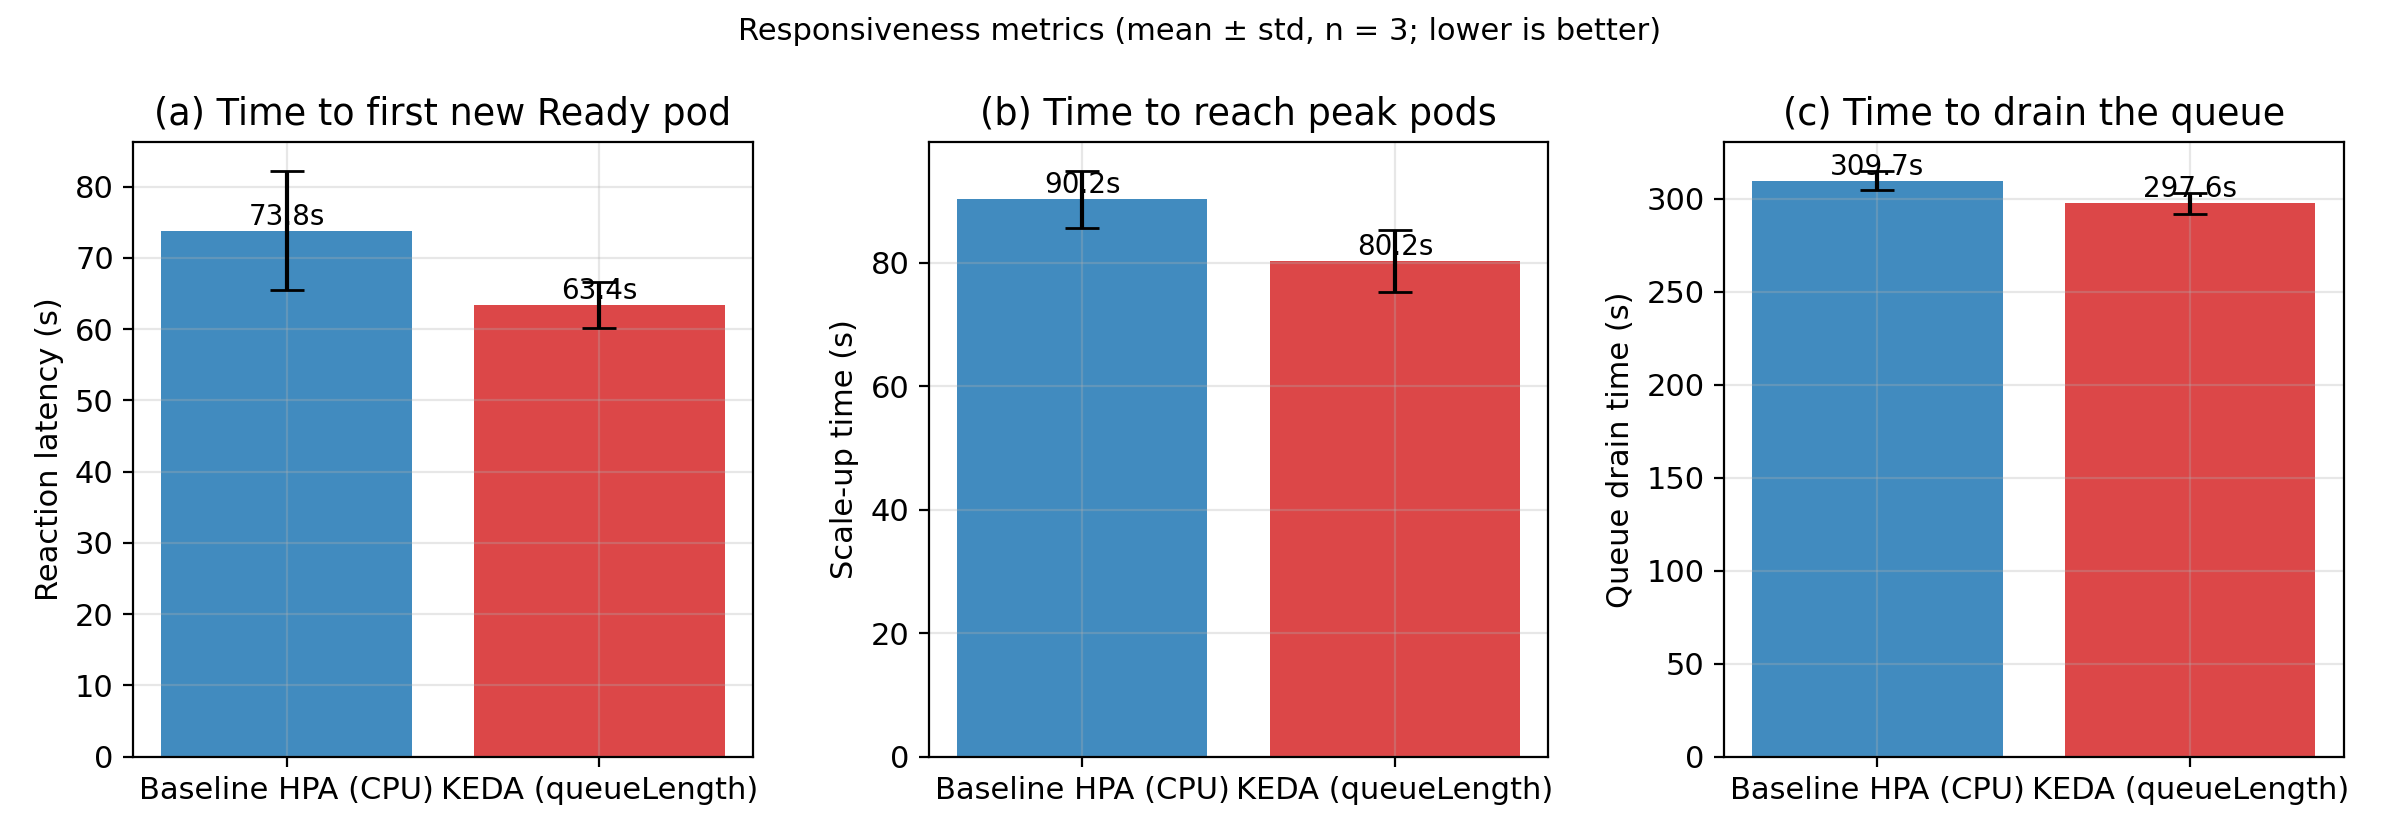
\includegraphics[width=0.93\linewidth]{../results/figures/fig4-response-bar.png}
  \caption{Responsiveness metrics. KEDA responds earlier because queue length is visible as soon as backlog forms, while CPU-based HPA waits for resource metrics to cross the target.}
  \label{fig:response}
\end{figure}

The per-run timeline figures in \texttt{results/figures/} show the same pattern in every matched run. KEDA reaches 5--6 Ready pods first, its queue-depth curve stays below the baseline HPA during the drain, and only KEDA removes pods before the trial ends. The aggregate bar chart therefore reflects a consistent run-level pattern rather than a single outlier.

\subsection{Scale-down Behaviour}
\label{subsec:res-scaledown}
The strongest qualitative difference appears after the burst stops. Fig.~\ref{fig:scaledown} shows that the baseline HPA does not scale down in any trial, while KEDA starts removing pods about 327~s after the burst ends and reaches three Ready pods by the end of the observation window. This is notable because both strategies use the same 60~s scale-down stabilisation window and the same 50\%/60~s removal policy.

\begin{figure}[t]
  \centering
  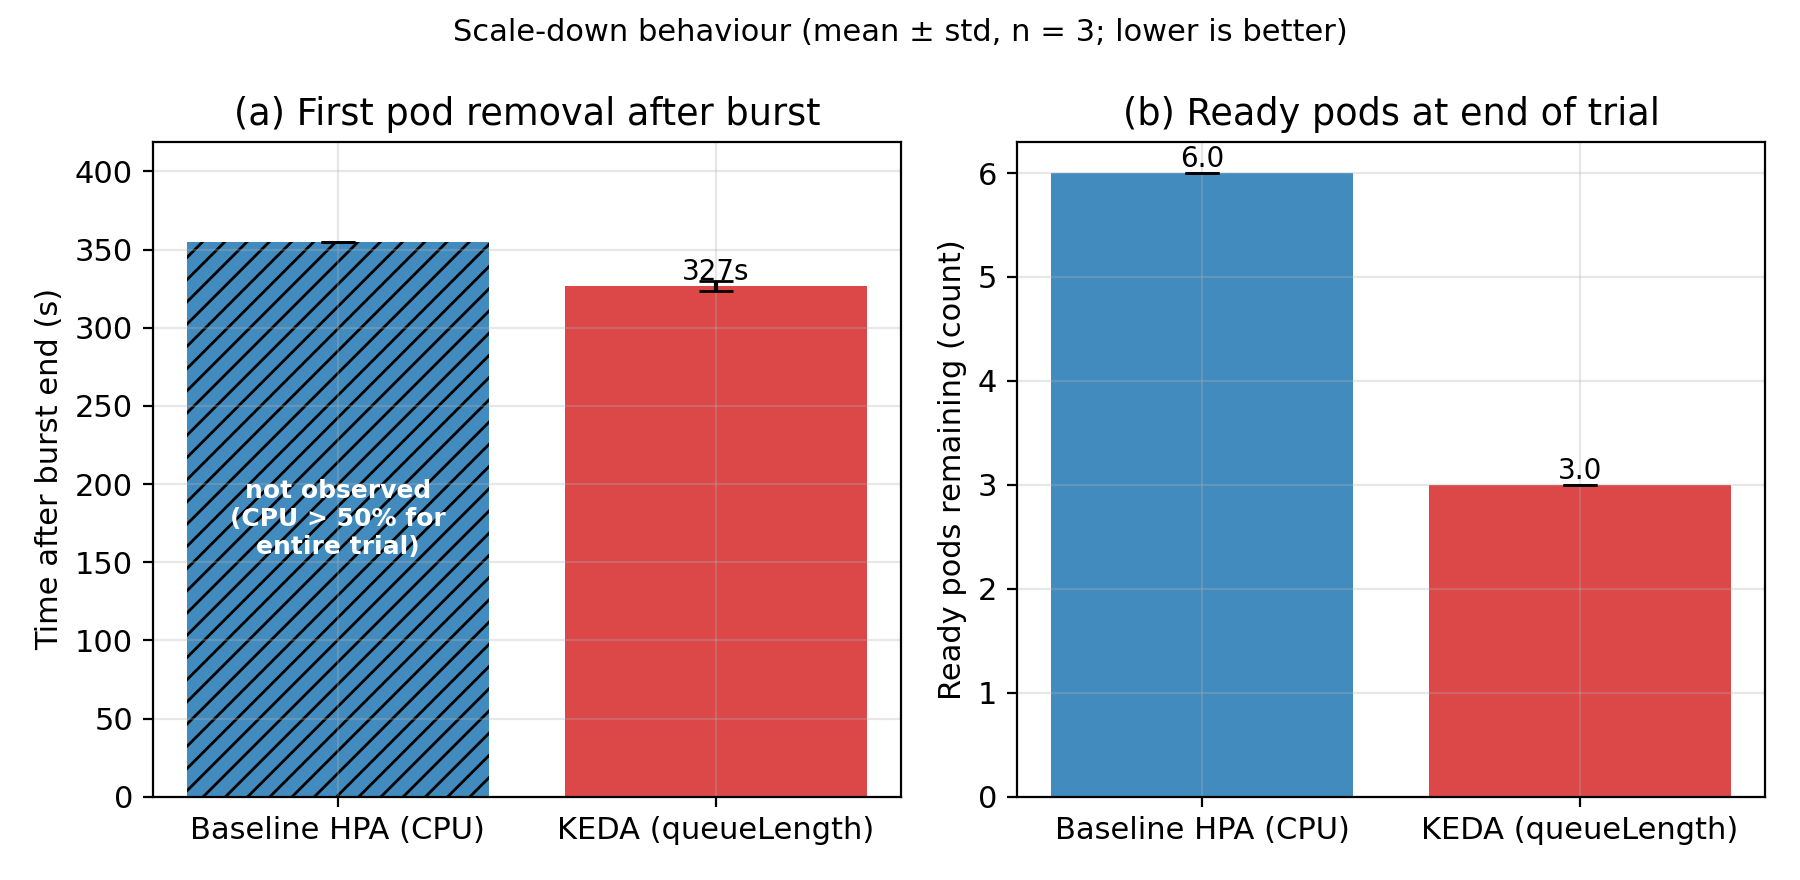
\includegraphics[width=0.93\linewidth]{../results/figures/fig5-scale-down-bar.png}
  \caption{Scale-down behaviour. The CPU-based HPA remains at six pods during the trial, while KEDA begins returning capacity once queue depth falls sufficiently.}
  \label{fig:scaledown}
\end{figure}

\textbf{Why HPA cannot shrink in the observed window.} The consumer is CPU-bound, and each pod is limited to 300~m CPU while requesting 100~m. As long as a pod has messages to process, it can remain close to the CPU limit. The HPA therefore observes utilisation near $300\%$ of the CPU request, far above the 50\% target. Substituting that ratio into Eq.~\ref{eq:hpa} keeps the desired replica count clamped at \texttt{maxReplicas}=6 until the queue is almost empty. In other words, the CPU signal tells HPA that the pods are busy, but it does not tell HPA that the backlog is already shrinking.

\textbf{Why KEDA shrinks earlier.} KEDA observes the queue directly. With the target $T=100$ messages per replica, the desired replica count decreases as $Q$ decreases. Once the queue has dropped far enough, KEDA can recommend fewer than six pods, and the shared 60~s stabilisation window delays but does not prevent the downscale. This is the key technical lesson of the experiment: using an event signal changes not only scale-up timing but also the ability to detect when extra capacity is no longer needed.

\subsection{Resource Cost Interpretation}
\label{subsec:res-cost}
The pod-seconds overshoot is similar for the two strategies: $1\,426 \pm 27$ for HPA and $1\,415 \pm 7$ for KEDA. This does not contradict the scale-down result. Both strategies quickly reach the same six-pod cap, and most of the trial is spent processing the burst, so the cost curves are similar over this short window. KEDA's cost advantage appears in the tail because it starts returning pods earlier. A longer post-drain observation period would likely enlarge the pod-seconds gap.

\section{Discussion}
\label{sec:discussion}

\paragraph{The signal matters more than the parameters.}~The most
consequential finding of this study is that KEDA's advantage is
rooted in \emph{what} it measures rather than in \emph{how} the
underlying HPA control block is configured. Both scalers were given
an identical $60$\,s stabilisation window, an identical
\texttt{Percent 50\%/60s} scale-down policy, and an identical scale-up
budget; only the signal differed. Operators tempted to tune the HPA
\texttt{behavior} block in an attempt to recover KEDA's observed
responsiveness are therefore optimising a second-order variable.

\paragraph{Why CPU fails on queue-backed workloads.}~For a
CPU-bound consumer governed by a strict \texttt{limits.cpu}, the CPU
signal saturates the moment the queue has any residual work: the
reported utilisation becomes the ratio of limit to request,
independent of the backlog. The HPA can thus neither \emph{estimate}
the deficit while the burst is active nor \emph{release} capacity
while the drain is still in flight. Queue length, in contrast, is a
direct measurement of outstanding work and carries both pieces of
information simultaneously.

\paragraph{When HPA remains reasonable.}~For synchronous HTTP services
without an intermediate queue, CPU remains a plausible scaling signal
and the HPA's simplicity is attractive. For queue consumers, a hybrid
policy is often the pragmatic production choice: let queue length drive
normal elasticity and retain CPU-based limits as a guardrail against
runaway scale-up.

\paragraph{Limitations and next steps.}~The study is confined to a
single-node cluster, one EC2 instance type, one broker, and three
replications per group; it therefore demonstrates a clear directional
effect rather than a universal law. The $\approx\,355$\,s post-burst
window also truncates the Baseline HPA's scale-down tail, so the
observed cost gap is conservative. Future work should sweep
\texttt{cpu} and queue-length targets, compare against HPA with native
\texttt{External} metrics, and repeat the study on multi-node clusters.

\section{Conclusion}
\label{sec:conclusion}

This project implemented a controlled technical evaluation of CPU-based HPA and queue-length-based KEDA for the same RabbitMQ-backed Spring Boot consumer on Kubernetes. With all non-signal parameters held constant, KEDA reacted 10.4~s faster, reached peak capacity earlier, drained the queue 12.2~s sooner, and scaled down during the observation window while HPA stayed at six pods. The reason is that queue length measures unfinished work directly, whereas CPU mainly shows that the current pods are busy. For event-driven cloud workloads, choosing the right autoscaling signal is therefore more important than only tuning the HPA behaviour parameters.


% --- References ---------------------------------------------------------
\bibliographystyle{IEEEtran}
\bibliography{references}

% --- Artifact Appendix (does not count towards the 9-page limit) --------
\clearpage
\appendix
\section*{Artifact Appendix}
\addcontentsline{toc}{section}{Artifact Appendix}

\subsection*{A.1 Artifact Overview}
This appendix describes how to reproduce the project. The artifact contains the Spring Boot consumer, RabbitMQ and Kubernetes manifests, HPA and KEDA scaling policies, Python load-generation scripts, shell scripts for deployment and data collection, raw experimental CSV files, and Python analysis scripts that regenerate the figures and summary table.

\subsection*{A.2 Hardware and Software Dependencies}
\begin{itemize}
  \item \textbf{Cloud host}: AWS EC2 \texttt{m5.large} with Ubuntu~22.04~LTS. A \texttt{t3.medium} can be used for smoke testing, but the reported experiments use \texttt{m5.large}.
  \item \textbf{Cluster stack}: K3s v1.30, Helm~3, \texttt{metrics-server} v0.7, KEDA v2.13, and RabbitMQ \texttt{3.12-management}.
  \item \textbf{Build tools}: Java~17, Maven~3.9, Docker~24.x or compatible Docker Buildx environment.
  \item \textbf{Load-test tools}: Python~3.10+ with \texttt{pika}, \texttt{click}, and \texttt{PyYAML} as listed in the load-test requirements file.
  \item \textbf{Analysis tools}: Python~3.10+ with \texttt{pandas} and \texttt{matplotlib} as listed in the analysis requirements file.
\end{itemize}

\subsection*{A.3 Repository}
The public repository is:
\begin{center}
\url{https://github.com/QinHaoting/CS5296-Group5-Autoscaling}
\end{center}

Key directories are:
\begin{itemize}
  \item \texttt{consumer/}: Spring Boot RabbitMQ consumer.
  \item \texttt{k8s/}: namespaces, RabbitMQ, HPA baseline, and KEDA manifests.
  \item \texttt{load-test/}: workload producer and YAML traffic patterns.
  \item \texttt{scripts/}: setup, deployment, collection, run, and teardown scripts.
  \item \texttt{results/}: raw CSV data, generated figures, and \texttt{summary.csv}.
  \item \texttt{analysis/}: scripts for metric extraction and plotting.
\end{itemize}

\subsection*{A.4 Build and Deployment}
\begin{enumerate}
  \item Build and push the consumer image:
\begin{verbatim}
docker buildx build --platform linux/amd64 \
  -t <dockerhub>/cs5296-consumer:v1.0 --push consumer/
\end{verbatim}
  \item On the EC2 node, install the cluster dependencies and base services:
\begin{verbatim}
bash scripts/setup.sh
\end{verbatim}
  \item Deploy both experiment groups:
\begin{verbatim}
export CONSUMER_IMAGE=<dockerhub>/cs5296-consumer:v1.0
bash scripts/deploy-baseline.sh
bash scripts/deploy-keda.sh
\end{verbatim}
  \item Confirm that RabbitMQ, the consumers, HPA, and KEDA are running:
\begin{verbatim}
kubectl get pods -A
kubectl -n baseline get hpa
kubectl -n keda get scaledobject,hpa
\end{verbatim}
\end{enumerate}

\subsection*{A.5 Running the Experiments}
Run one trial for each strategy:
\begin{verbatim}
bash scripts/run-experiment.sh baseline 1
bash scripts/run-experiment.sh keda 1
\end{verbatim}

Run the full three-trial batch:
\begin{verbatim}
for run in 1 2 3; do bash scripts/run-experiment.sh baseline "$run"; done
for run in 1 2 3; do bash scripts/run-experiment.sh keda "$run"; done
\end{verbatim}

Each trial resets the Deployment to one replica, purges the target queue, records a short baseline, runs the burst producer, and keeps collecting metrics during the post-burst drain period. The full six-trial batch takes about 49 minutes, excluding manual setup time.

\subsection*{A.6 Reproducing the Figures}
After the raw CSV files exist, regenerate the summary and figures with:
\begin{verbatim}
python analysis/plot.py
\end{verbatim}
Expected outputs include \texttt{summary.csv}, three per-run timeline figures, and the aggregate figures for responsiveness, scale-down behaviour, and pod-seconds overshoot.

\subsection*{A.7 Expected Results}
The regenerated \texttt{summary.csv} should show that KEDA reacts approximately 10~s faster than the CPU-based HPA, drains the queue approximately 12~s sooner, and triggers scale-down during the trial. The exact numbers may vary slightly with EC2 performance, RabbitMQ startup time, and producer-side timing, but the qualitative result should remain: queue-length-based scaling reacts earlier and releases capacity earlier for this queue-backed workload.

\subsection*{A.8 Troubleshooting}
Additional operational notes are in \texttt{docs/RUNBOOK.md}. Common checks include verifying the RabbitMQ NodePort, confirming that the two queues are empty before each trial, ensuring \texttt{metrics-server} is reporting CPU metrics, and checking that the KEDA \texttt{ScaledObject} has an active RabbitMQ trigger.


\end{document}
